\section{Synthesis and research agenda}

The evidence points to three connected changes. First, ABM has expanded across health, ecology, mobility, cities, energy, opinion, and policy, particularly where heterogeneous individuals interact within coupled systems. Second, LLMs are entering the modeling process both inside agents’ behavioral and decision mechanisms and as tools for coding, data work, analysis, and interfaces. Third, collaboration has become more extensive and international, while research remains divided among specialized communities.

\begin{figure}[htbp]
\centering
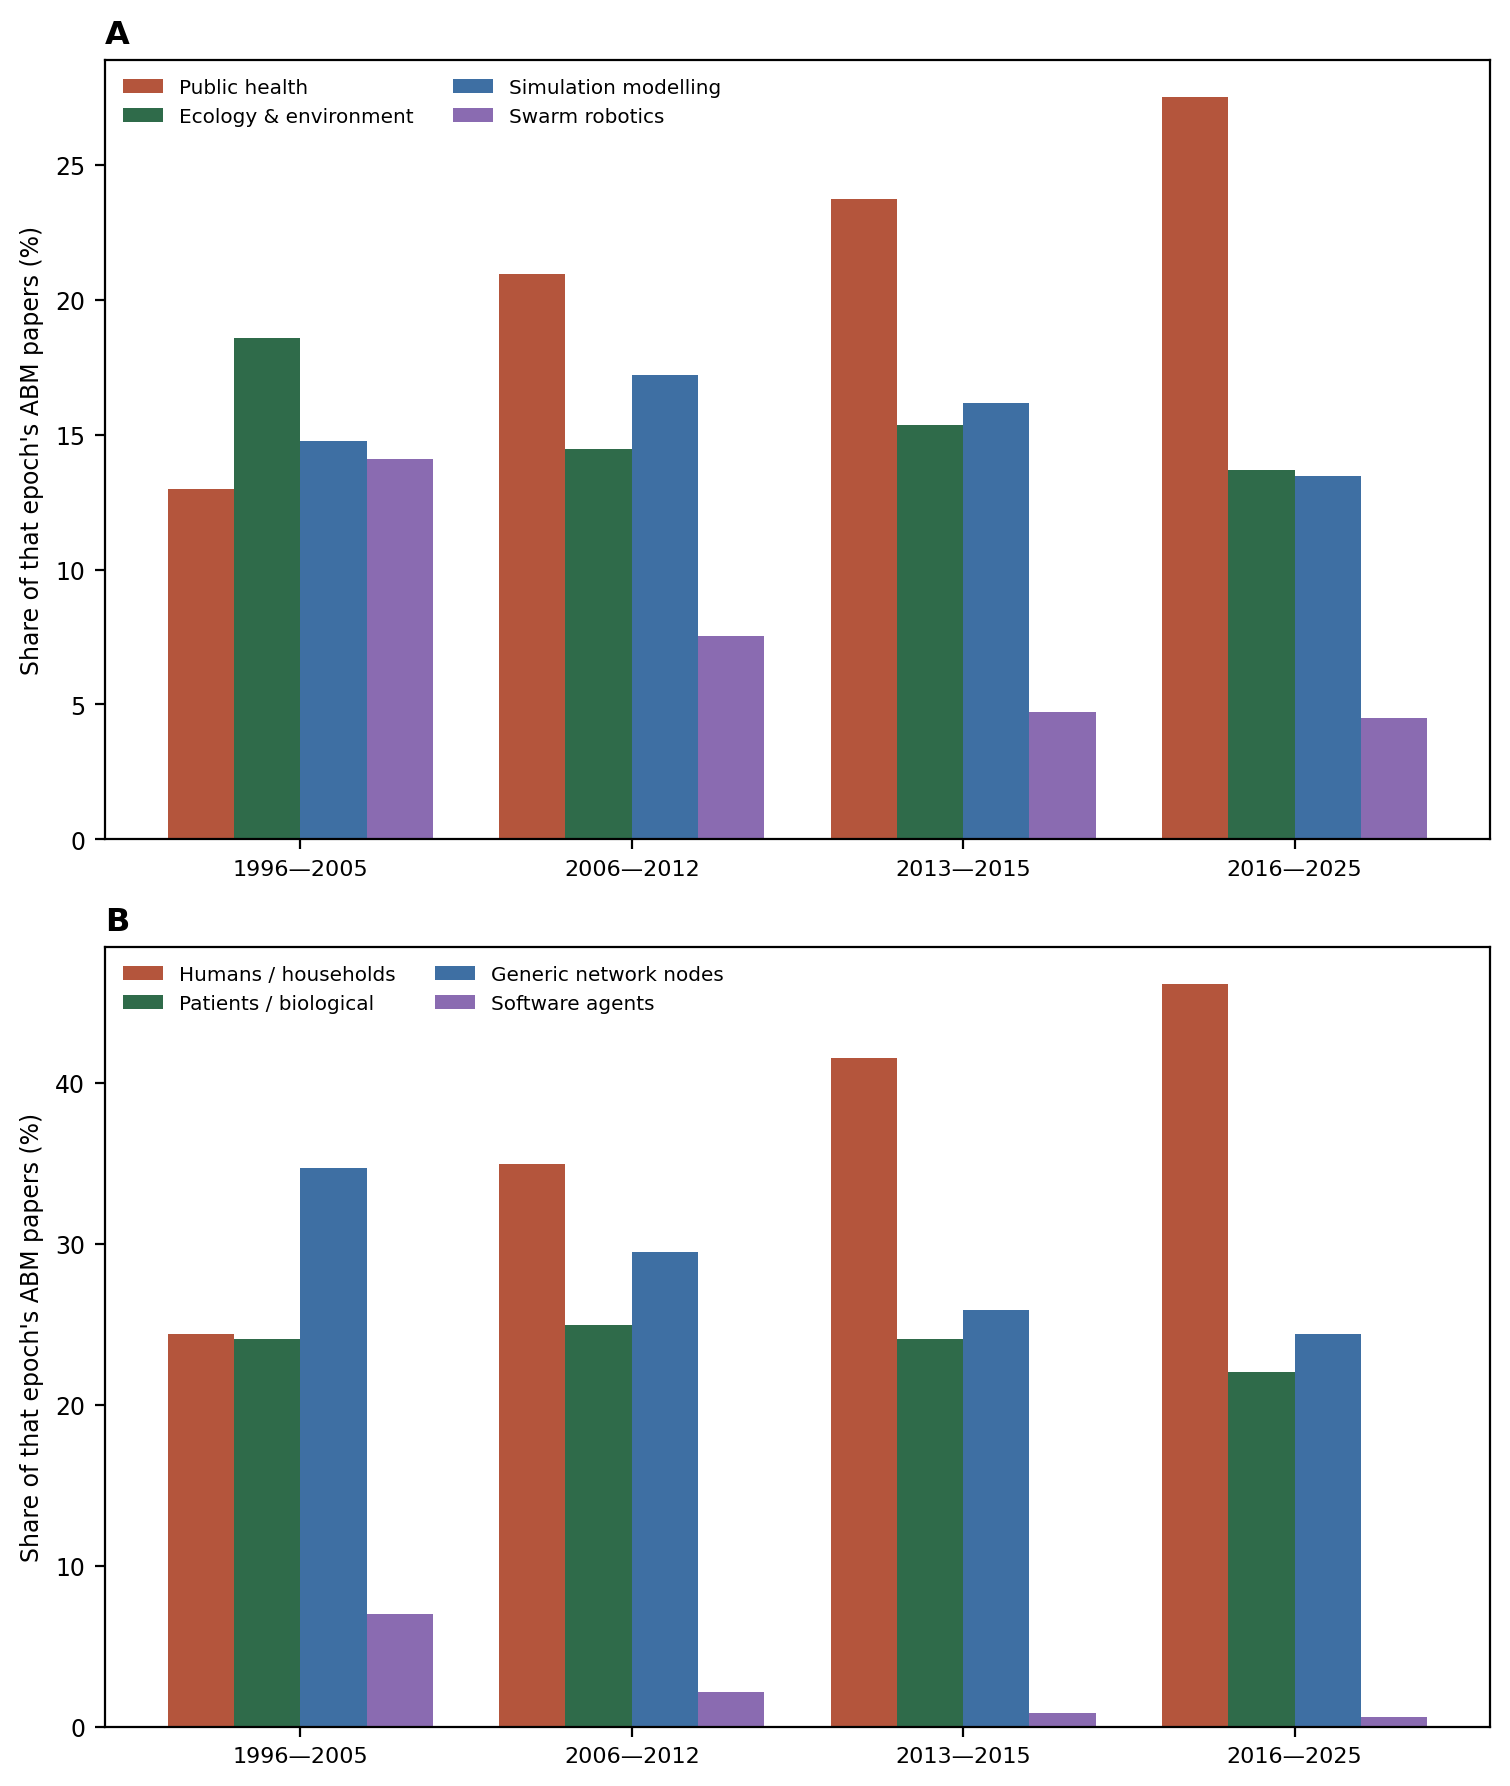
\includegraphics[width=0.88\textwidth,height=0.78\textheight,keepaspectratio]{figures/figure_20.png}
\setcounter{figure}{21}
\caption{Temporal evolution of research topics and modeled agent types.}
\label{fig:figure22}
\end{figure}

These changes are best understood as interdependent rather than sequential. Broader applications create demand for richer behavioral mechanisms; richer mechanisms heighten the need for empirical validation and shared standards; and the collaboration network shapes how those standards spread. The central question is therefore not whether LLMs will replace conventional ABM, but whether the field can incorporate generative decision mechanisms without sacrificing transparency, calibration, and reproducibility.

This synthesis yields five priorities. First, evaluate behavior against empirical benchmarks rather than conversational plausibility alone. Second, report the LLM’s function and position in the model, distinguishing internal decision mechanisms from supporting uses. Third, extend ODD-style reporting to include prompts, model versions, seeds, memory, retrieval, and safeguards. Fourth, develop cross-domain benchmarks that connect epidemiology, mobility, social influence, and policy models. Fifth, examine collaboration networks as channels of methodological diffusion, including whether LLM-enabled papers bridge existing groups or form a weakly connected cluster.

\begin{figure}[htbp]
\centering
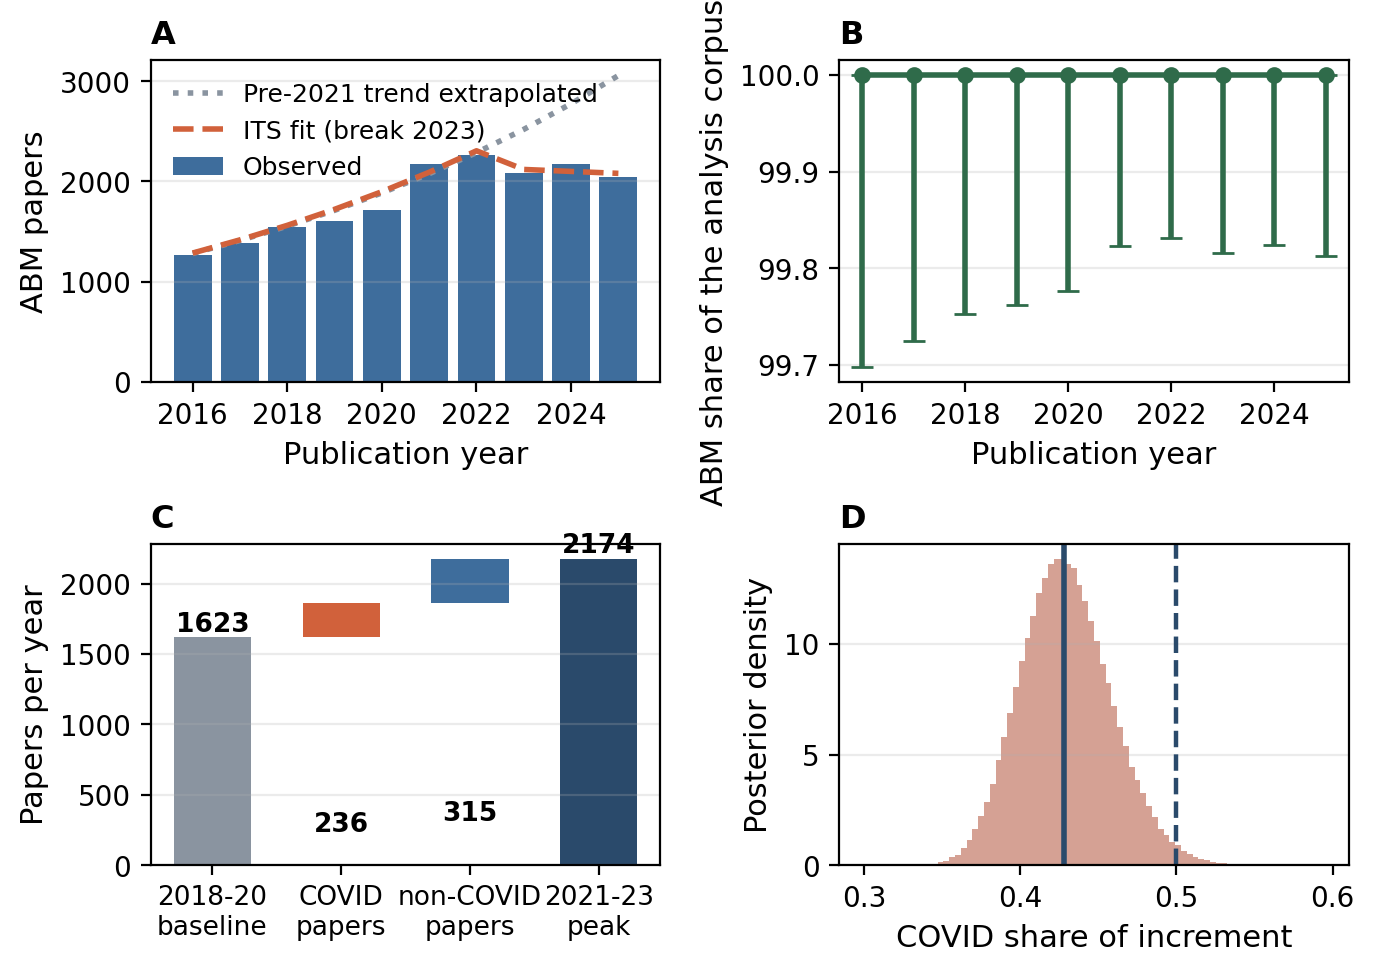
\includegraphics[width=0.88\textwidth,height=0.78\textheight,keepaspectratio]{figures/figure_21.png}
\setcounter{figure}{22}
\caption{Statistical examination of the 2021–2023 publication peak: breakpoint, ABM share, decomposition, and posterior distribution.}
\label{fig:figure23}
\end{figure}